\section{\texorpdfstring{\gls{ml}}{ML} Model}\label{sec:ML}
After the creation of the dataset, the main machine learning machine was trained and tested.

This remaining part has been developed on a Jupyter notebook, publicly available on Github and Kaggle alongside the dataset used.
\begin{itemize}
    \item Github repo: \url{https://github.com}
    \item Kaggle repo: \url{https://www.kaggle.com}
\end{itemize}
\subsection{Dataset analysis}
The dataset used has \texttt{7000} entries in total, each one representing a simulated motor.

Thanks to the various libraries used, it was possible to analyze data using intuitive graphical plots.
\subsubsection{Frequency plot}
\begin{figure}[H]
    \centering
    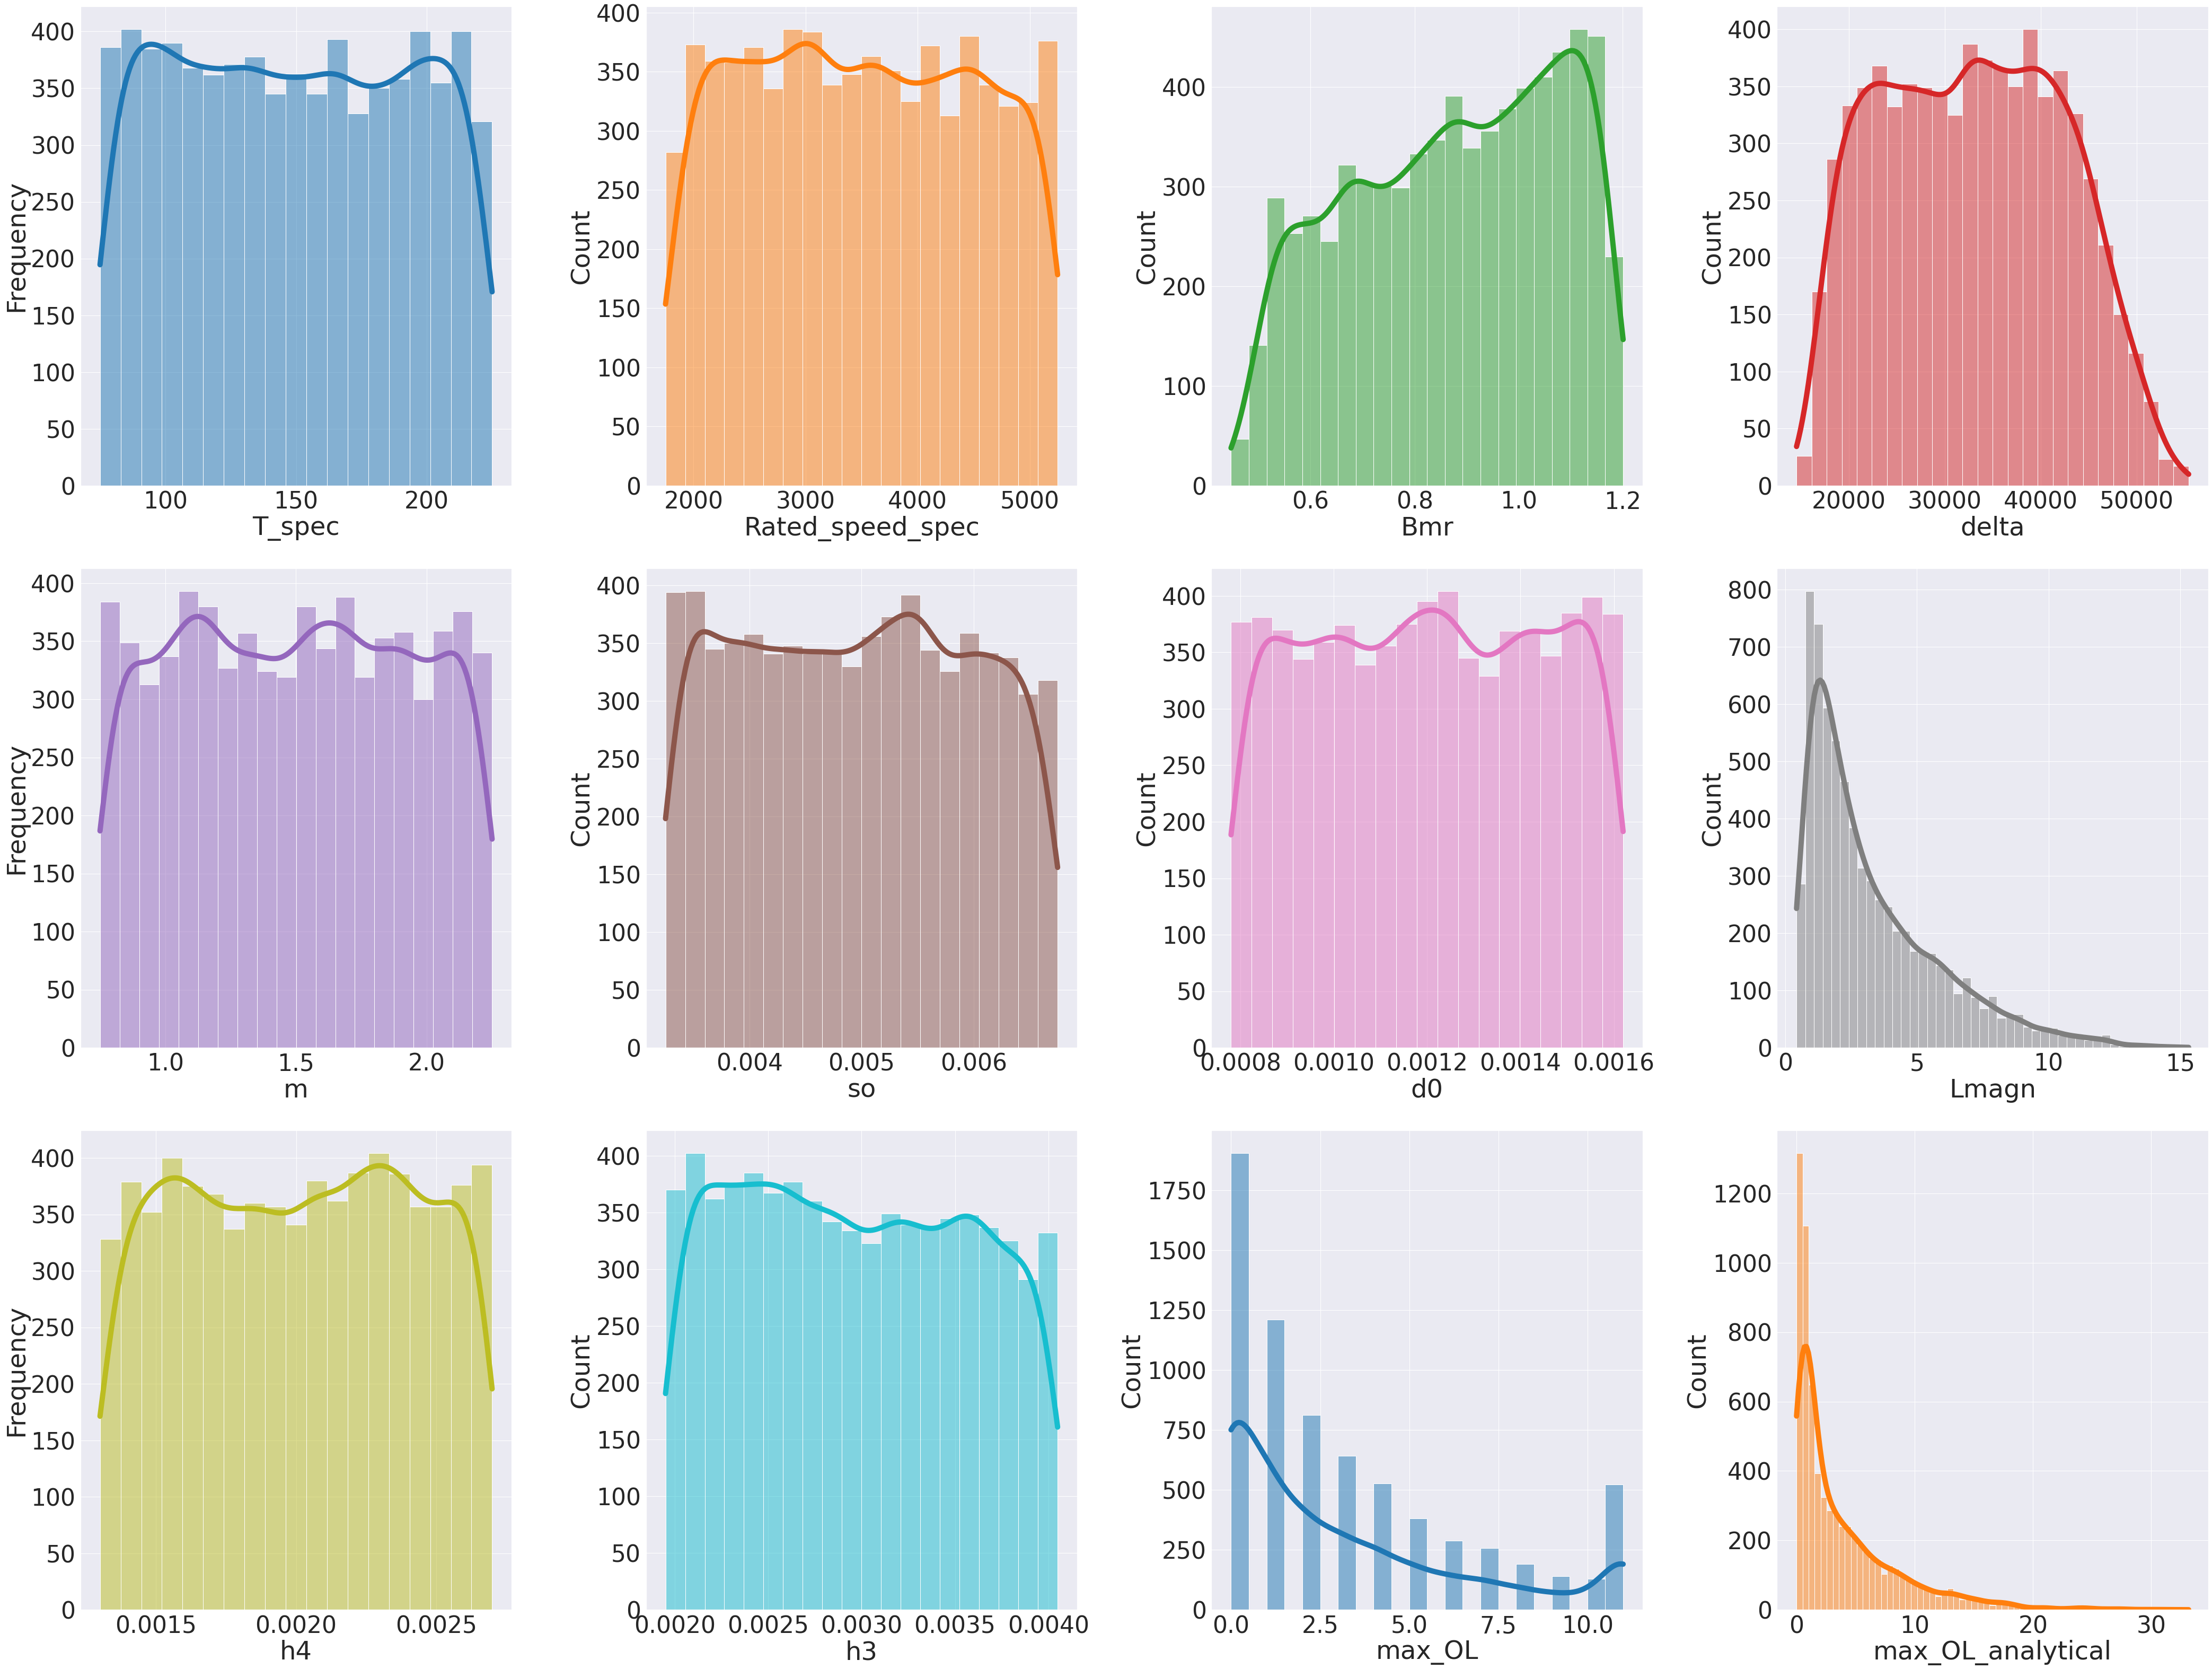
\includegraphics[width=0.6\textwidth]{sections/images/section3/frequency_plot.png}
    \caption{Frequency plot}
    \label{fig:freq_plot}
\end{figure}
The frequency plot in \cref{fig:freq_plot} shows that all the labels are randomly distributed, except fot the magnet height $L_{magn}$.

The last two plots, shows the distribution of \gls{fem} and analytical prediction.
\subsubsection{Correlation Matrix}
\begin{figure}[H]
    \centering
    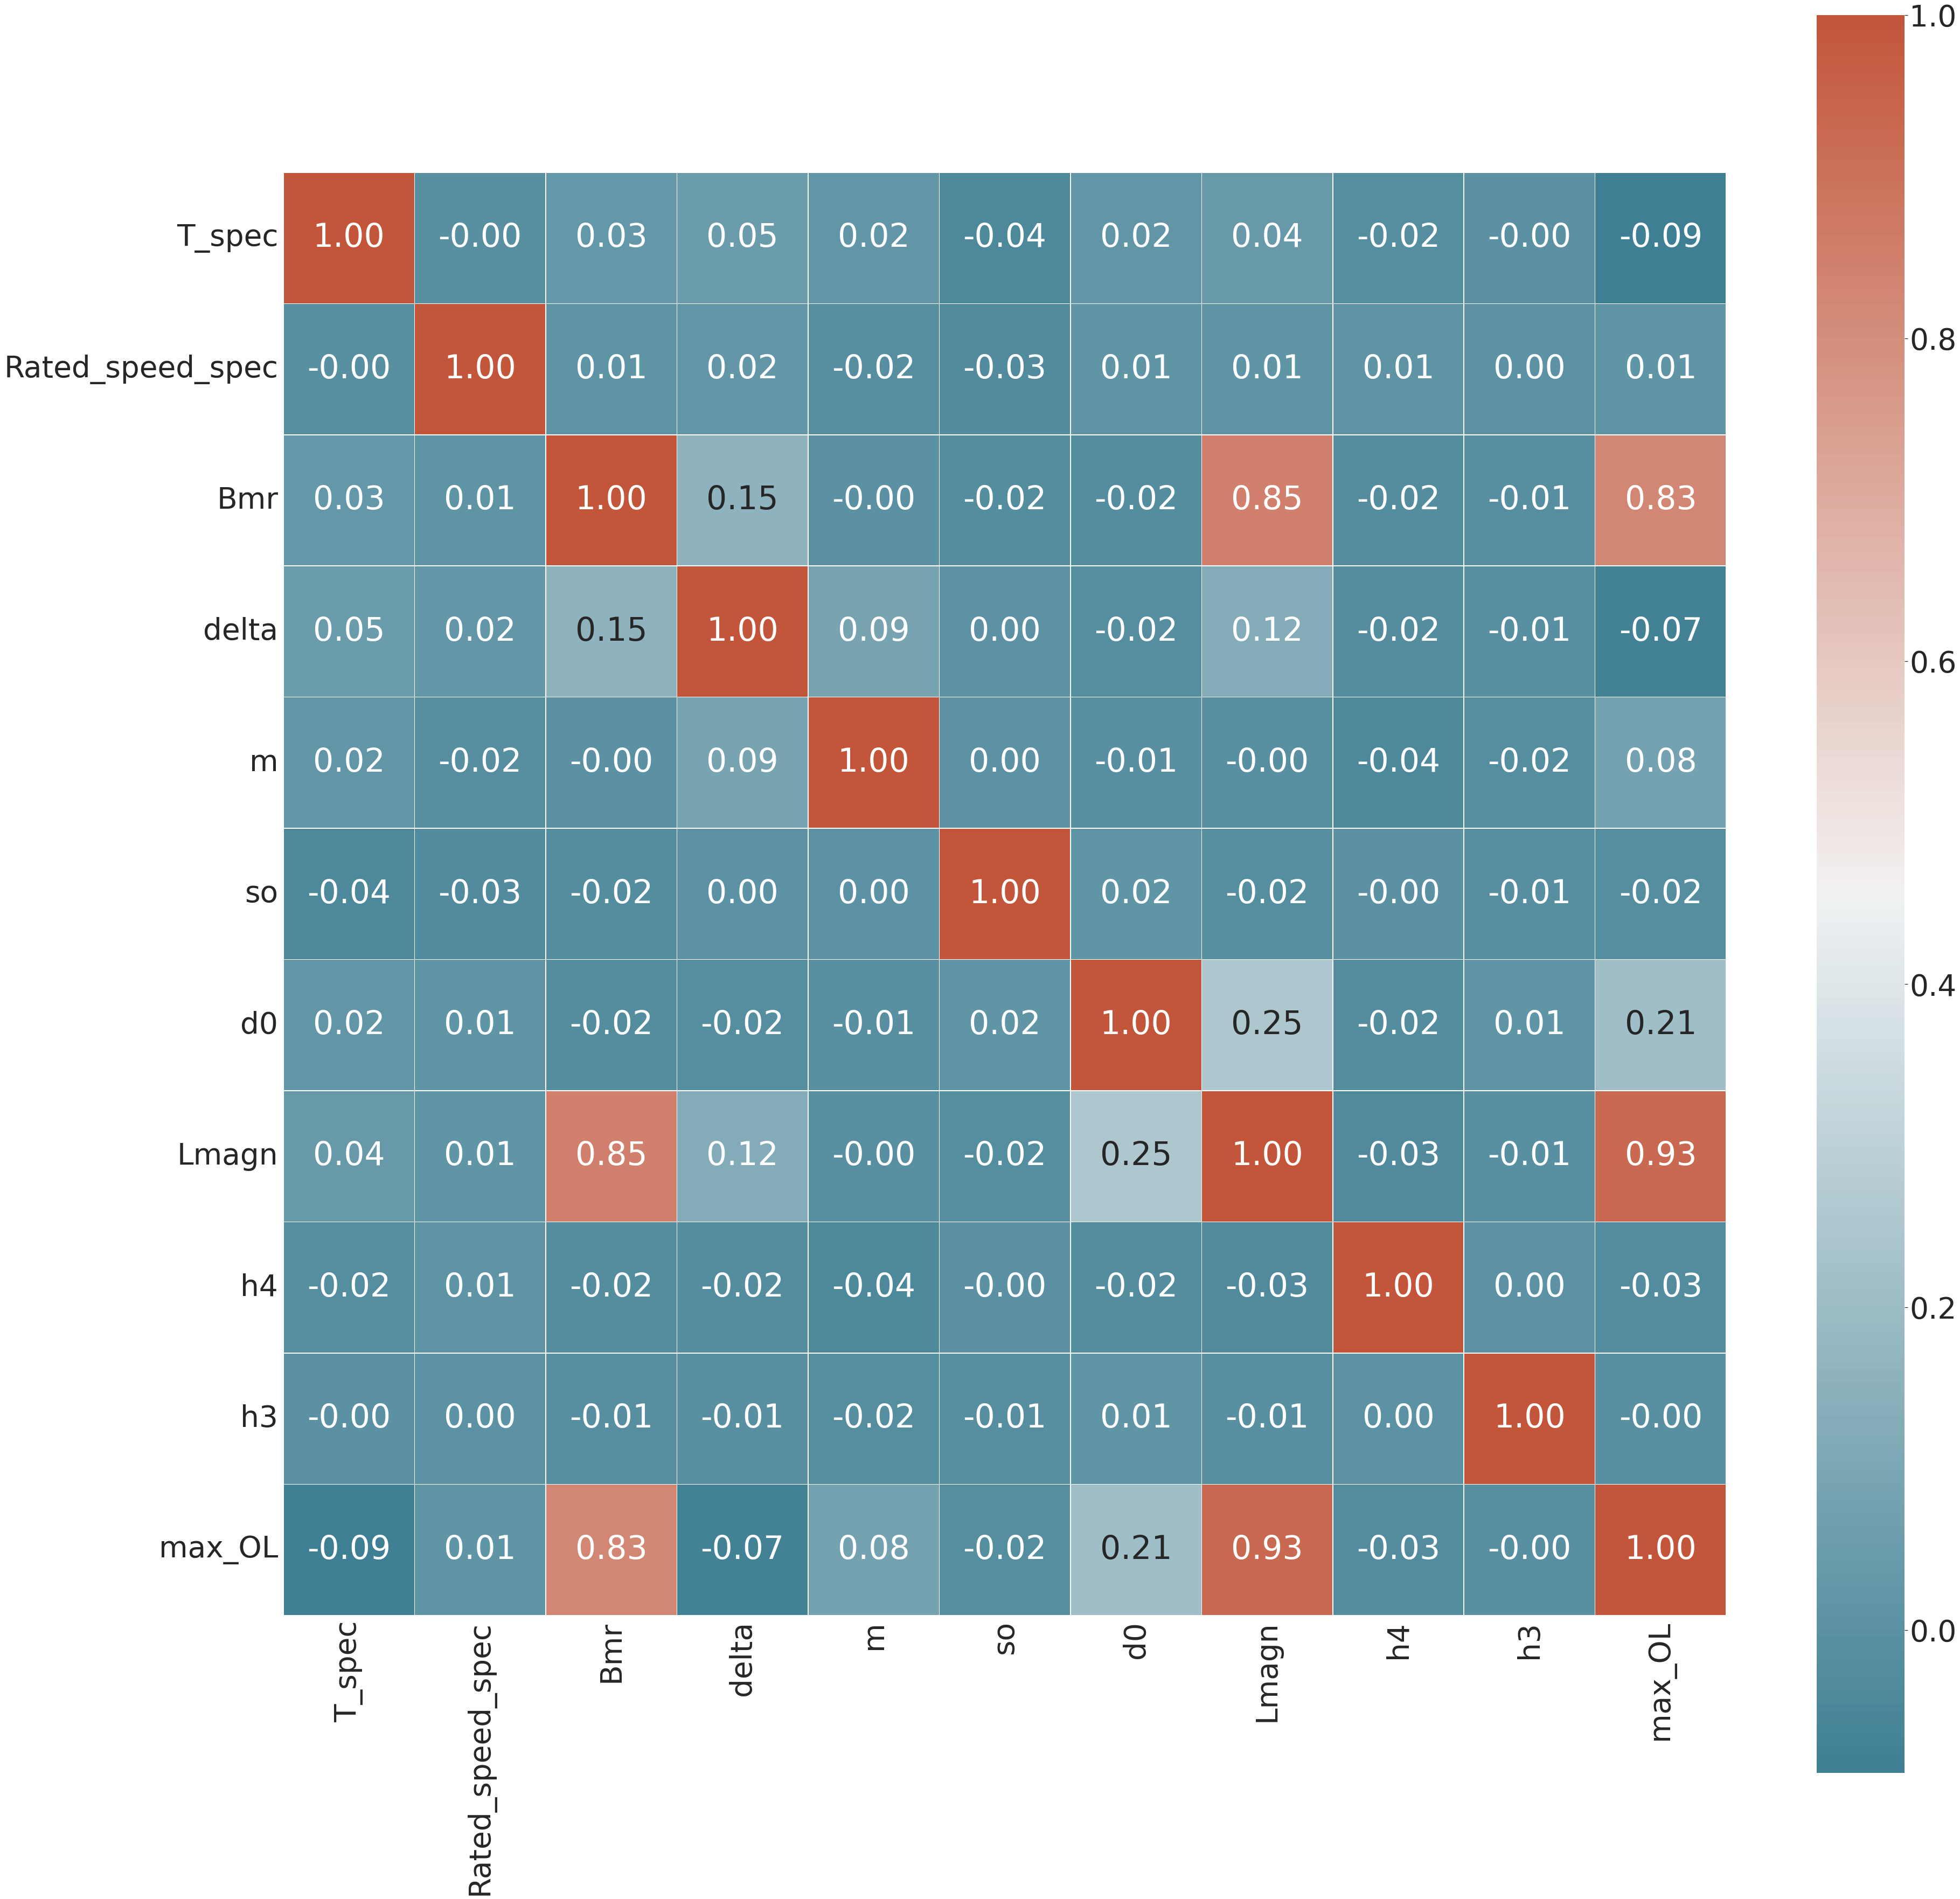
\includegraphics[width=0.6\textwidth]{sections/images/section3/correlation_matrix.png}
    \caption{Correlation Matrix}
    \label{fig:corr_matrix}
\end{figure}
As it is possible to see from the correlation matrix in \cref{fig:corr_matrix}, the magnet height $L_{magn}$ and the magnetic loading $B_{mr}$ are highly correlated with the maximum overload.
\subsubsection{Dataset Split}
The dataset was split in three different set: 
\begin{itemize}
    \item Train set: used to train the Machine.
    \item Test set: Used for the final evaluation of the Machine.
    \item Validation set: used to validate the Machine during the training.
\end{itemize}
\subsubsection{Stratification}
Stratification is used to be sure that the proportion of labels in the sample produced will be the same as the proportion of labels in the dataset. This will increase the reproducibility.
\subsection{Metrics}
There are different metrics useful to identify a good model.

Those metrics have been introduced for binary classification, but it is possible to extend those to multi class.
Notation:
\begin{itemize}
    \item $TP$: True Positive.
    \item $TN$: True Negative.
    \item $FP$: False Positive.
    \item $FN$: False Negative.
\end{itemize}
\subsubsection{Precision}
Number of items correctly identified as positive out of the total items identified as positive:
\begin{equation}
    \frac{TP}{TP+FP}
\end{equation}
\subsubsection{Recall}
Number of items correctly identified as positive out of the total actual positives:
\begin{equation}
    \frac{TP}{TP+FN}
\end{equation}
\subsubsection{Accuracy}
Number of items correctly identified as either truly positive or truly negative out of the total number of items:
\begin{equation}
    \frac{TP+TN}{TP+TN+FP+FN}
\end{equation}
Usually it is the most used metrics for a first evaluation of the model.
\subsubsection{F1-Score}
The harmonic average of the precision and recall, it measures the effectiveness of identification when just as much importance is given to recall as to precision:
\begin{equation}
    \frac{TP+TN}{TP+TN+FP+FN}
\end{equation}
In multiclass, it can be calculated as an average of all the F1 score, or as a weighted average. Weights can be the number of samples for each category.
\subsubsection{Loss}
Loss is a number indicating how bad the model's prediction was on a single example. It is very important because it is the number that a model should seek to minimize during training.

Usually \gls{mse} is used as the loss function for regression:
\begin{equation}
    MSE=\frac{1}{N}\sum_{(x,y)\in D}\left(y-Prediction(x)\right)^2
\end{equation}
In multiclass classification, categorical Crossentropy is the most used:
\begin{equation}
    CrossEntropyLoss=-(y_i\log(\hat{y}_i)+(1-y_i)\log(1-\hat{y}_i))
\end{equation}
\subsection{Regression model}
The first machine trained is a linear regression model, that uses one or multiple parameters. The decision to use such simple machine is to start by using something simple and understandable, and it is interesting to see how performance increases by introducing complexity on the machine.
\subsubsection{Linear regression - one variable}
In order to train such machine with one variable, we need to chose a suitable feature that is going to weight a lot on the output label. In \cref{fig:corr_matrix} it is possible to see that $L_{magn}$ is the most correlated to the label, so that feature has chosen.
The trained model can be summarized as follows:
\begin{lstlisting}[basicstyle=\ttfamily\footnotesize]
Model: "sequential"
_________________________________________________________________
    Layer (type)                Output Shape              Param #   
=================================================================
    flatten (Flatten)           (None, 1)                 0         
                                                                    
    dense (Dense)               (None, 1)                 2         
                                                                    
=================================================================
Total params: 2
Trainable params: 2
Non-trainable params: 0
_________________________________________________________________
\end{lstlisting}
Information about the training:
\begin{center}
    \begin{table}[H]
       \renewcommand{\arraystretch}{1.2}
        \centerline{
        \centering
        \begin{tabular}{|r|c|c|c|}
        \hline
        Optimizer &epoch & loss  & metrics \\
        \hline
        Adam & $150$ & mean\_absolute\_error&accuracy\\
        \hline
        \end{tabular}}
    \end{table}
\end{center}
The result of this machine can be visualized in \cref{fig:linear_one_veariable}, and its result metrics are:
\begin{center}
    \begin{table}[H]
       \renewcommand{\arraystretch}{1.2}
        \centerline{
        \centering
        \begin{tabular}{|c|c|}
        \hline
        Validation loss &Validation accuracy \\
        \hline
        $0.8425$ & $0.3482$ \\
        \hline
        \end{tabular}}
    \end{table}
\end{center}
\begin{figure}[H]
    \centering
    \makebox[\textwidth][c]{
    %
    \begin{subfigure}{0.55\textwidth}
        \centering
        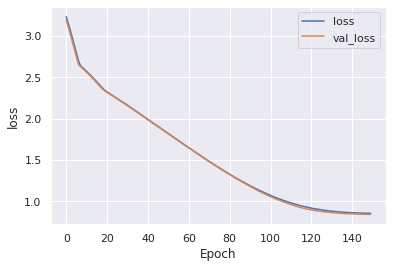
\includegraphics[width=.9\linewidth]{sections/images/section3/linear_one_veariable_loss.png}
        \caption{loss}
    \end{subfigure}
    %
    \begin{subfigure}{0.55\textwidth}
        \centering
        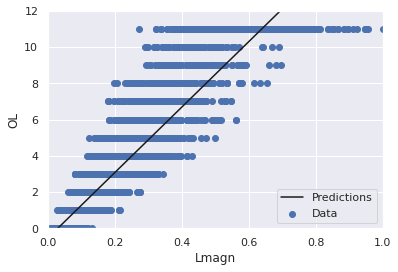
\includegraphics[width=.9\linewidth]{sections/images/section3/linear_one_veariable_plot.png}
        \caption{plot}
    \end{subfigure}}
  \caption{Linear regression - one variable}
  \label{fig:linear_one_veariable}
\end{figure}
%%%%%%%%%%%%%%%%%%%%%%%%%%%%%%%%%%%%%%%%%%%%%%%%%%%%%%%%%%%%%%%%%%%%%%%%%%%
\subsubsection{Linear regression - multi variable}
Now the linear regression machine have all the features in input, so we except to have better metrics.
The trained model can be summarized as follows:
\begin{lstlisting}[basicstyle=\ttfamily\footnotesize]
Model: "sequential"
_________________________________________________________________
    Layer (type)                Output Shape              Param #   
=================================================================
    flatten (Flatten)           (None, 10)                0         
                                                                    
    dense (Dense)               (None, 1)                 11        
                                                                    
=================================================================
Total params: 11
Trainable params: 11
Non-trainable params: 0
_________________________________________________________________
\end{lstlisting}
Information about the training:
\begin{center}
    \begin{table}[H]
       \renewcommand{\arraystretch}{1.2}
        \centerline{
        \centering
        \begin{tabular}{|r|c|c|c|}
        \hline
        Optimizer &epoch & loss  & metrics \\
        \hline
        Adam & $150$ & mean\_absolute\_error&accuracy\\
        \hline
        \end{tabular}}
    \end{table}
\end{center}
The result of this machine can be visualized in \cref{fig:linear_multi_veariable}, and its result metrics are:
\begin{center}
    \begin{table}[H]
       \renewcommand{\arraystretch}{1.2}
        \centerline{
        \centering
        \begin{tabular}{|c|c|}
        \hline
        Validation loss &Validation accuracy \\
        \hline
        $0.6756$ & $0.4089$ \\
        \hline
        \end{tabular}}
    \end{table}
\end{center}
\begin{figure}[H]
    \centering
    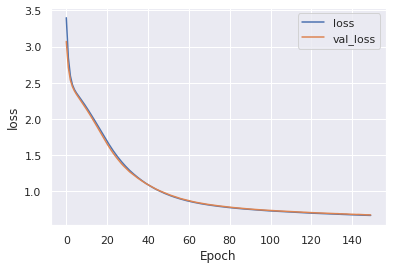
\includegraphics[width=.5\linewidth]{sections/images/section3/linear_multi_veariable.png}
    \caption{Linear regression - one variable - loss}
    \label{fig:linear_multi_veariable}
\end{figure}
%%%%%%%%%%%%%%%%%%%%%%%%%%%%%%%%%%%%%%%%%%%%%%%%%%%%%%%%%%%%%%%%%%
\subsubsection{NON Linear regression - one variable \texorpdfstring{$L_{magn}$}{Lmagn}}
$L_{magn}$ is again the feature used to train this one variable regression, but now a non linear regression will be used.
A \gls{dnn} has been used to create this non linear regression machine.
The trained model can be summarized as follows:
\begin{lstlisting}[basicstyle=\ttfamily\footnotesize]
Model: "sequential"
_________________________________________________________________
    Layer (type)                Output Shape              Param #   
=================================================================
    flatten (Flatten)           (None, 1)                 0         
                                                                    
    dense (Dense)               (None, 32)                64        
                                                                    
    dense_1 (Dense)             (None, 64)                2112      
                                                                    
    dense_2 (Dense)             (None, 128)               8320      
                                                                    
    dense_3 (Dense)             (None, 1)                 129       
                                                                    
=================================================================
Total params: 10,625
Trainable params: 10,625
Non-trainable params: 0
_________________________________________________________________
\end{lstlisting}
Information about the training:
\begin{center}
    \begin{table}[H]
       \renewcommand{\arraystretch}{1.2}
        \centerline{
        \centering
        \begin{tabular}{|r|c|c|c|}
        \hline
        Optimizer &epoch & loss  & metrics \\
        \hline
        Adam & $150$ & mean\_absolute\_error&accuracy\\
        \hline
        \end{tabular}}
    \end{table}
\end{center}
The result of this machine can be visualized in \cref{fig:non_linear_one_veariable}, and its result metrics are:
\begin{center}
    \begin{table}[H]
       \renewcommand{\arraystretch}{1.2}
        \centerline{
        \centering
        \begin{tabular}{|c|c|}
        \hline
        Validation loss &Validation accuracy \\
        \hline
        $0.7681$ & $0.3518$ \\
        \hline
        \end{tabular}}
    \end{table}
\end{center}
\begin{figure}[H]
    \centering
    \makebox[\textwidth][c]{
    %
    \begin{subfigure}{0.55\textwidth}
        \centering
        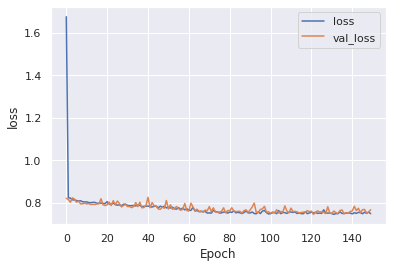
\includegraphics[width=.9\linewidth]{sections/images/section3/non_linear_one_veariable_loss.png}
        \caption{loss}
    \end{subfigure}
    %
    \begin{subfigure}{0.55\textwidth}
        \centering
        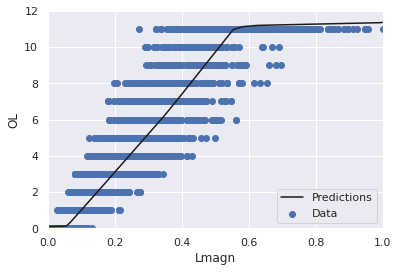
\includegraphics[width=.9\linewidth]{sections/images/section3/non_linear_one_veariable_plot.png}
        \caption{plot}
    \end{subfigure}}
  \caption{NON Linear regression - one variable - $L_{magn}$}
  \label{fig:non_linear_one_veariable}
\end{figure}
%%%%%%%%%%%%%%%%%%%%%%%%%%%%%%%%%%%%%%%%%%%%%%%%%%%%%%%%%%%%%%%%%%
\subsubsection{NON Linear regression - one variable \texorpdfstring{$B_{mr}$}{Bmr}}
The \gls{dnn} non linear regression machine is the sames before, but now the feature used is $B_{mr}$: the second most relevant according to the correlation matrix (\cref{fig:corr_matrix}).
The trained model can be summarized as follows:
\begin{lstlisting}[basicstyle=\ttfamily\footnotesize]
Model: "sequential"
_________________________________________________________________
    Layer (type)                Output Shape              Param #   
=================================================================
    flatten (Flatten)           (None, 1)                 0         
                                                                    
    dense (Dense)               (None, 32)                64        
                                                                    
    dense_1 (Dense)             (None, 64)                2112      
                                                                    
    dense_2 (Dense)             (None, 128)               8320      
                                                                    
    dense_3 (Dense)             (None, 1)                 129       
                                                                    
=================================================================
Total params: 10,625
Trainable params: 10,625
Non-trainable params: 0
_________________________________________________________________
\end{lstlisting}
Information about the training:
\begin{center}
    \begin{table}[H]
       \renewcommand{\arraystretch}{1.2}
        \centerline{
        \centering
        \begin{tabular}{|r|c|c|c|}
        \hline
        Optimizer &epoch & loss  & metrics \\
        \hline
        Adam & $150$ & mean\_absolute\_error&accuracy\\
        \hline
        \end{tabular}}
    \end{table}
\end{center}
The result of this machine can be visualized in \cref{fig:non_linear_one_bmr_veariable}, and its result metrics are:
\begin{center}
    \begin{table}[H]
       \renewcommand{\arraystretch}{1.2}
        \centerline{
        \centering
        \begin{tabular}{|c|c|}
        \hline
        Validation loss &Validation accuracy \\
        \hline
        $1.0235$ & $0.3357$ \\
        \hline
        \end{tabular}}
    \end{table}
\end{center}
\begin{figure}[H]
    \centering
    \makebox[\textwidth][c]{
    %
    \begin{subfigure}{0.55\textwidth}
        \centering
        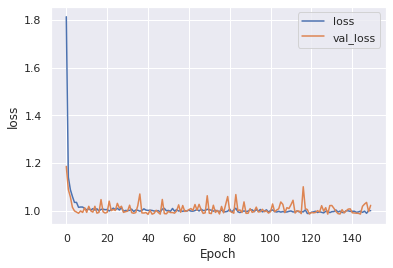
\includegraphics[width=.9\linewidth]{sections/images/section3/non_linear_one_veariable_bmr_loss.png}
        \caption{loss}
    \end{subfigure}
    %
    \begin{subfigure}{0.55\textwidth}
        \centering
        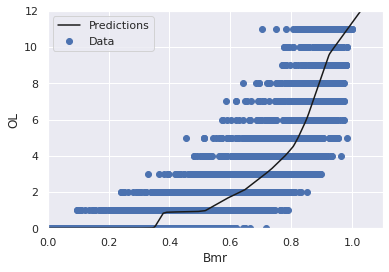
\includegraphics[width=.9\linewidth]{sections/images/section3/non_linear_one_veariable_bmr_plot.png}
        \caption{plot}
    \end{subfigure}}
  \caption{NON Linear regression - one variable - $B_{mr}$}
  \label{fig:non_linear_one_bmr_veariable}
\end{figure}
%%%%%%%%%%%%%%%%%%%%%%%%%%%%%%%%%%%%%%%%%%%%%%%%%%%%%%%%%%%%%%%%%%%%%%%%%%%
\subsubsection{NON Linear regression - multi variable}
Now the non linear regression machine utilize in input all the features, so we except to have better metrics. The depth of the network is increased to try reaching an useful value of metrics. The trained model can be summarized as follows:
\begin{lstlisting}[basicstyle=\ttfamily\footnotesize]
Model: "sequential"
_________________________________________________________________
    Layer (type)                Output Shape              Param #   
=================================================================
    flatten (Flatten)           (None, 10)                0         
                                                                    
    dense (Dense)               (None, 32)                352       
                                                                    
    dense_1 (Dense)             (None, 64)                2112      
                                                                    
    dense_2 (Dense)             (None, 128)               8320      
                                                                    
    dense_3 (Dense)             (None, 256)               33024     
                                                                    
    dense_4 (Dense)             (None, 1)                 257       
                                                                    
=================================================================
Total params: 44,065
Trainable params: 44,065
Non-trainable params: 0
_________________________________________________________________
\end{lstlisting}
Information about the training:
\begin{center}
    \begin{table}[H]
       \renewcommand{\arraystretch}{1.2}
        \centerline{
        \centering
        \begin{tabular}{|r|c|c|c|}
        \hline
        Optimizer &epoch & loss  & metrics \\
        \hline
        Adam & $150$ & mean\_absolute\_error&accuracy\\
        \hline
        \end{tabular}}
    \end{table}
\end{center}
The result of this machine can be visualized in \cref{fig:non_linear_multi_veariable}, and its result metrics are:
\begin{center}
    \begin{table}[H]
       \renewcommand{\arraystretch}{1.2}
        \centerline{
        \centering
        \begin{tabular}{|c|c|}
        \hline
        Validation loss &Validation accuracy \\
        \hline
        $0.1590$ & $0.4339$ \\
        \hline
        \end{tabular}}
    \end{table}
\end{center}
\begin{figure}[H]
    \centering
    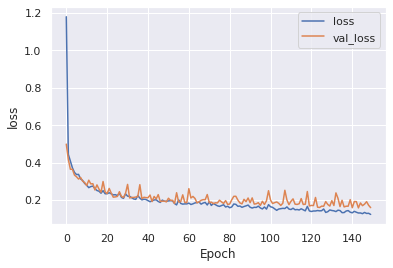
\includegraphics[width=.5\linewidth]{sections/images/section3/non_linear_multi_veariable_loss.png}
    \caption{non Linear regression - Multi variable - loss}
    \label{fig:non_linear_multi_veariable}
\end{figure}
Accuracy and loss are the highest until now, but are still unusable in real word applications.
%%%%%%%%%%%%%%%%%%%%%%%%%%%%%%%%%%%%%%%%%%%%%%%%%%%%%%%%%%%%%%%%%%%%%%%%%%%
\subsection{Classification \texorpdfstring{\glsxtrlong{dnn}}{Deep Neural Network}}
The machine using classification gives the best result for our problem, as it will be seen trough the metrics. The trained \gls{dnn} model has been chosen by a trial and error approach, and it is quite deep. The trained model can be summarized as follows:
\begin{lstlisting}[basicstyle=\ttfamily\footnotesize]
Model: "sequential"
_________________________________________________________________
    Layer (type)                Output Shape              Param #   
=================================================================
    flatten (Flatten)           (None, 10)                0         
                                                                    
    dense (Dense)               (None, 32)                352       
                                                                    
    dense_1 (Dense)             (None, 64)                2112      
                                                                    
    dense_2 (Dense)             (None, 128)               8320      
                                                                    
    dense_3 (Dense)             (None, 256)               33024     
                                                                    
    dense_4 (Dense)             (None, 12)                3084      
                                                                    
=================================================================
Total params: 46,892
Trainable params: 46,892
Non-trainable params: 0
_________________________________________________________________
\end{lstlisting}
Information about the training:
\begin{center}
    \begin{table}[H]
       \renewcommand{\arraystretch}{1.2}
        \centerline{
        \centering
        \begin{tabular}{|r|c|c|c|}
        \hline
        Optimizer &epoch & loss  & metrics \\
        \hline
        Adam & $150$ & SparseCategoricalCrossentropy&accuracy\\
        \hline
        \end{tabular}}
    \end{table}
\end{center}
The result of this machine can be visualized in \cref{fig:DNN_classification}, and its result metrics are:
\begin{center}
    \begin{table}[H]
       \renewcommand{\arraystretch}{1.2}
        \centerline{
        \centering
        \begin{tabular}{|c|c|}
        \hline
        Validation loss &Validation accuracy \\
        \hline
        $0.2841$ & $0.8893$ \\
        \hline
        \end{tabular}}
    \end{table}
\end{center}
\begin{figure}[H]
    \centering
    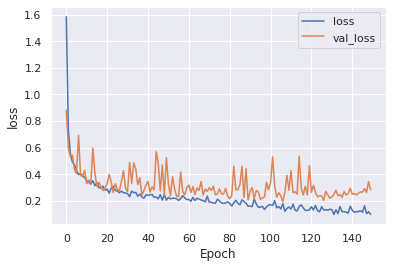
\includegraphics[width=.5\linewidth]{sections/images/section3/DNN_classification.png}
    \caption{\gls{dnn} Classification - loss}
    \label{fig:DNN_classification}
\end{figure}
\subsubsection{Evaluation with Test data}
It is assumed that it is the most performing network for our model, so it is suitable to evaluate it using the test data. The result metrics of the \gls{dnn} classification model are:
\begin{center}
    \begin{table}[H]
       \renewcommand{\arraystretch}{1.2}
        \centerline{
        \centering
        \begin{tabular}{|c|c|}
        \hline
        Validation loss &Validation accuracy \\
        \hline
        $0.2963$ & $0.9029$ \\
        \hline
        \end{tabular}}
    \end{table}
\end{center}
It can be seen that Loss increases compared with the non linear regression - multi variable. This is excepted because regression take in consideration the distance between output and labels more than a classification, and our problem is more prone to regression by design.

\textbf{NOTE:} comparing two losses, having different loss functions (like in this case) is not completely correct. Accuracy should be used instead.

Other metrics can be obtained, like the Precision, Recall and f1-score:
\begin{lstlisting}[basicstyle=\ttfamily\footnotesize]
              precision    recall  f1-score   support
       
           0      0.979     0.987     0.983       381
           1      0.950     0.938     0.944       242
           2      0.929     0.883     0.905       162
           3      0.836     0.953     0.891       128
           4      0.812     0.867     0.839       105
           5      0.789     0.737     0.762        76
           6      0.811     0.741     0.775        58
           7      0.766     0.706     0.735        51
           8      0.737     0.737     0.737        38
           9      0.793     0.821     0.807        28
          10      0.724     0.808     0.764        26
          11      1.000     0.933     0.966       105

    accuracy                          0.903      1400
   macro avg      0.844     0.843     0.842      1400
weighted avg      0.904     0.903     0.903      1400
\end{lstlisting}
Another interesting plot to see is the confusion matrix in \cref{fig:confusion_matrix}. It can give an intuitive idea on the precision and loss of the network by using colors.
\begin{figure}[H]
    \centering
    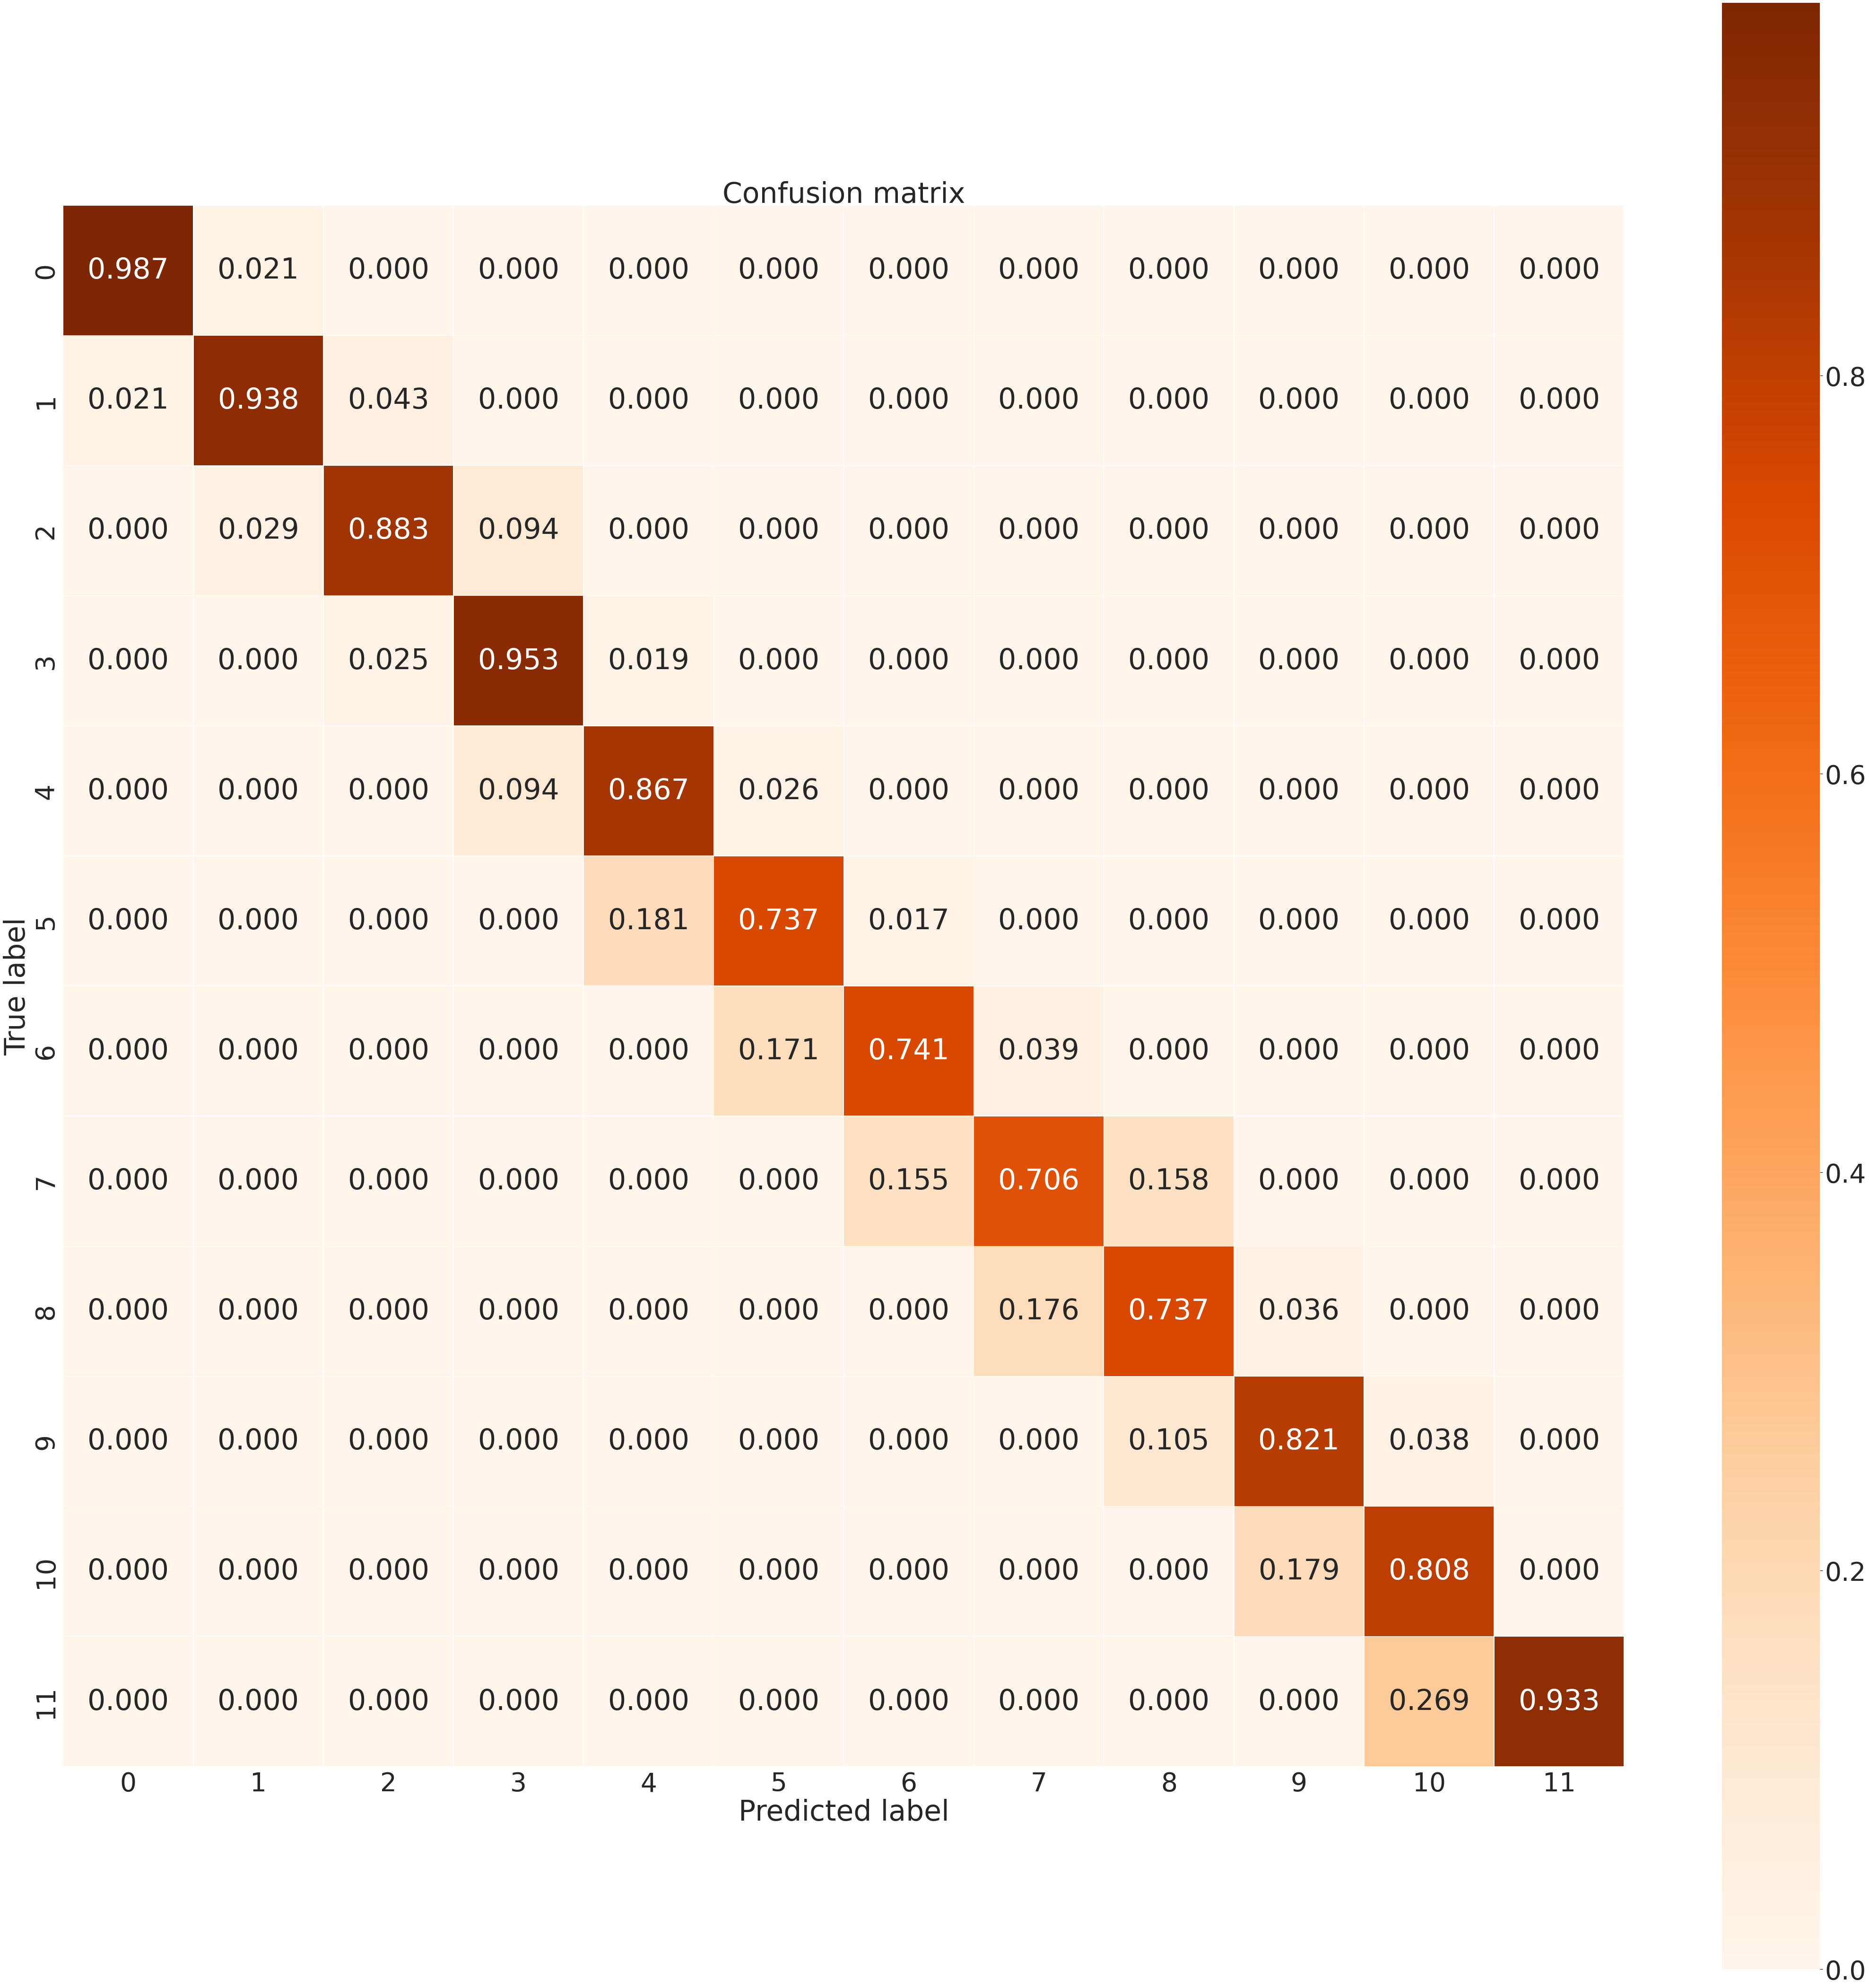
\includegraphics[width=.6\linewidth]{sections/images/section3/confusion_matrix.png}
    \caption{\gls{dnn} Classification - Confusion Matrix}
    \label{fig:confusion_matrix}
\end{figure}
\subsection{Comparison with analytical formula}
It is possible to use the analytical formula in \cref{eq:demagn_formula_approx} to predict the maximum overload. As already discussed, it is a simplified formula, and worse accuracy is excepted.

The same dataset of $7000$ samples has been used, and then the result of the function was rounded with different rounding method. Rounding is needed to make the analytical and \gls{ml} results comparable by the same metrics (accuracy).

The used rounding method are
\begin{itemize}
    \item \emph{Nearest}: rounds the number to the closest integer.
    \item \emph{Ceil}: rounds a number to the closest integer value larger than the current number.
    \item \emph{Floor}: rounds the integer to the closest integer smaller than the current one.
\end{itemize}

The resulting accuracy of the formula with different rounding methods is shown on the following table:
\begin{center}
    \begin{table}[H]
       \renewcommand{\arraystretch}{1.2}
        \centerline{
        \centering
        \begin{tabular}{|c|c|}
        \hline
        Rounding method &Accuracy \\
        \hline
        Nearest & $0.588$ \\
        \hline
        Ceil & $0.240$ \\
        \hline
        Floor  & $0.685$ \\
        \hline
        \end{tabular}}
    \end{table}
\end{center}
The floor rounding got the best accuracy, the analysis will be focusing on it. Confusion matrix of the analytical model using floor rounding can be seen in \cref{fig:confusion_matrix_analytical}. Precision, Recall and f1-score are the following:
\begin{lstlisting}[basicstyle=\ttfamily\footnotesize]
              precision    recall  f1-score   support

           0      0.722     0.901     0.801      1903
           1      0.520     0.454     0.485      1211
           2      0.815     0.608     0.697       812
           3      0.945     0.783     0.857       641
           4      0.911     0.759     0.828       526
           5      0.721     0.692     0.706       380
           6      0.609     0.581     0.595       289
           7      0.413     0.377     0.394       257
           8      0.239     0.277     0.257       191
           9      0.177     0.209     0.191       139
          10      0.261     0.281     0.271       128
          11      0.826     0.937     0.878       523

    accuracy                          0.685      7000
   macro avg      0.597     0.572     0.580      7000
weighted avg      0.692     0.685     0.682      7000
\end{lstlisting}
\begin{figure}[H]
    \centering
    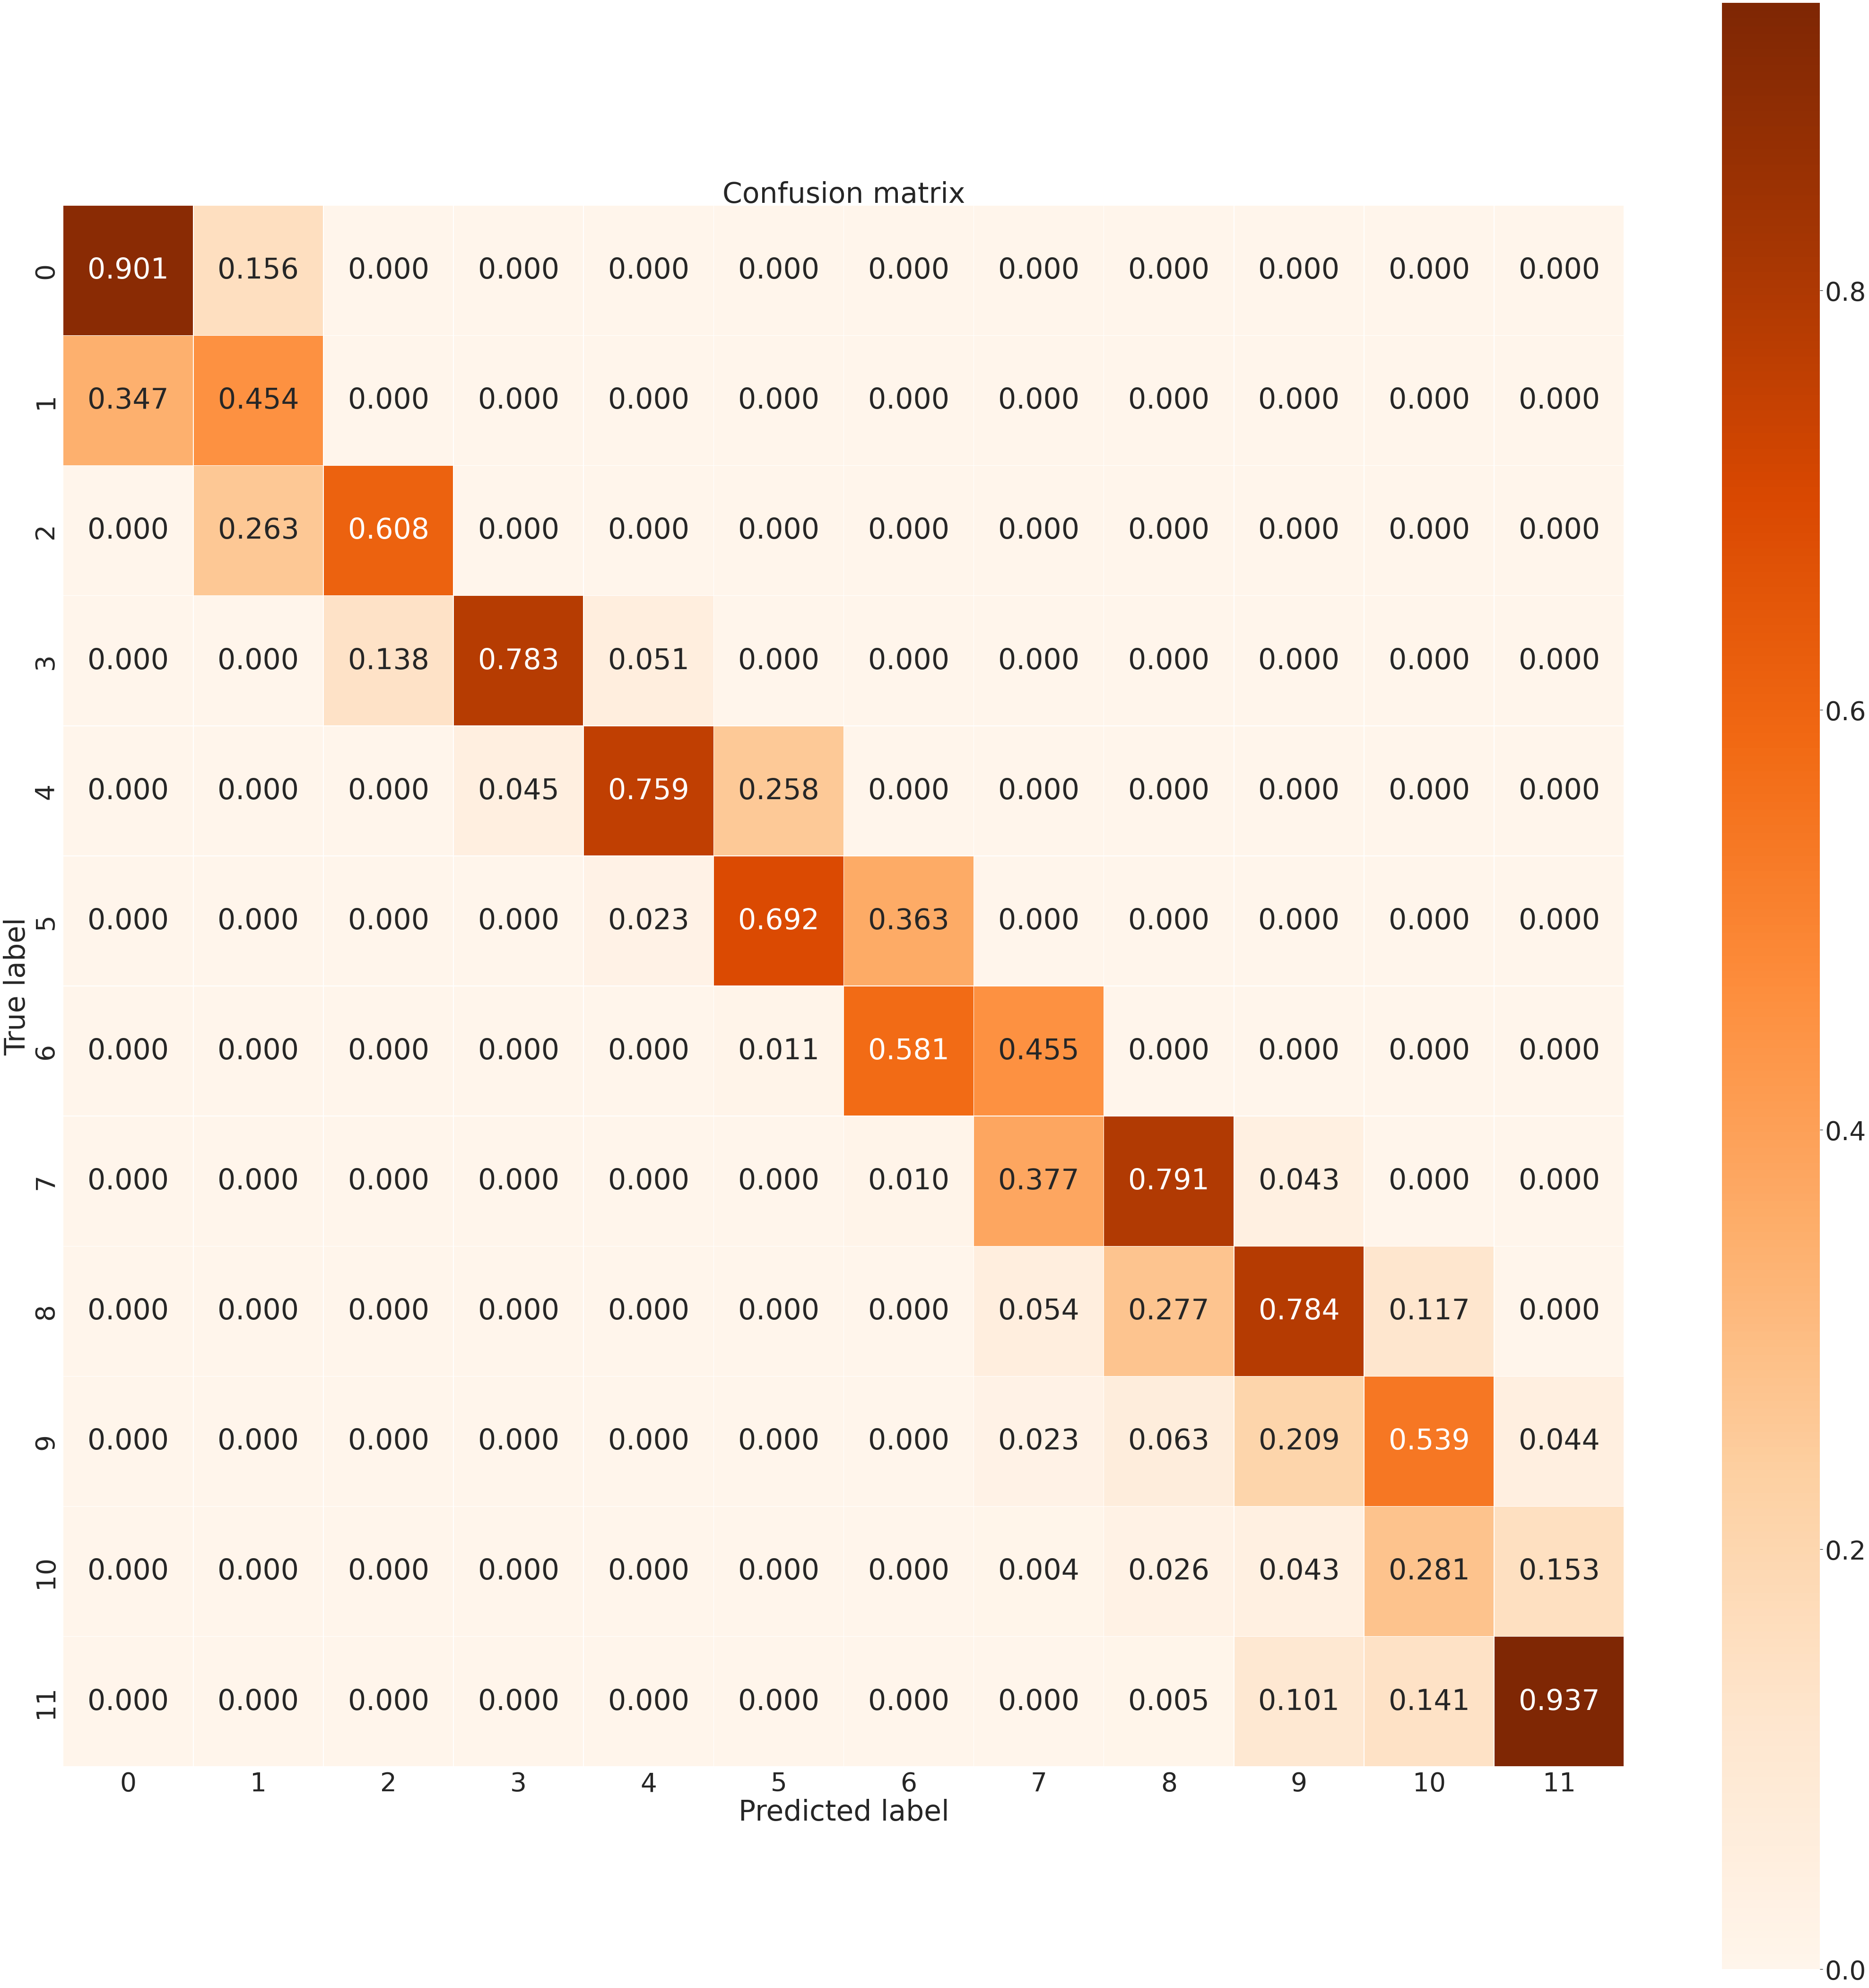
\includegraphics[width=.6\linewidth]{sections/images/section3/confusion_matrix_analytical.png}
    \caption{Analytical Model - Confusion Matrix}
    \label{fig:confusion_matrix_analytical}
\end{figure}
\section{Results, future works and improvements}
In the following table, all the interesting result metrics can be appreciated:
\begin{center}
    \begin{table}[H]
       \renewcommand{\arraystretch}{1.2}
        \centerline{
        \centering
        \begin{tabular}{|l|c|c|}
        \hline
        &Validation loss &Validation accuracy \\
        \hline
        Linear regression - one variable&$0.8425 $ & $0.3482$ \\
        \hline
        Linear regression - multi variable&$0.6756 $ & $0.4089$ \\
        \hline
        NON Linear regression - one variable $L_{magn}$&$0.7681 $ & $0.3518$ \\
        \hline
        NON Linear regression - one variable $B_{mr}$&$1.0235 $ & $0.3357$ \\
        \hline
        NON Linear regression - multi variable &$0.1590 $ & $0.4339$ \\
        \hline
        \gls{dnn} classification model&$0.2841 $ & $0.8893$ \\
        \hline
        Analytical Equation&$--$ & $0.685$ \\
        \hline
        \end{tabular}}
    \end{table}
\end{center}
It can be seen that the \gls{dnn} classification model outperforms any other model used in this report. this work can be considered as a good start for \gls{ml} application in \gls{pmsm} demagnetization.

It is proper to remember that this model is strongly limited: only one type of motor is used, with limited amount motor specifications, and with fixed materials. A future work could be to extend the network, and make it work for more type of motors. Despite this limitation, it is possible to see how \gls{ml} can be successfully be used to speed up and improve electric motor design, that was the initial target of this work.

In \cref{fig:model_dnn}, the final network of the \gls{dnn} classifier.
\begin{figure}[H]
    \centering
    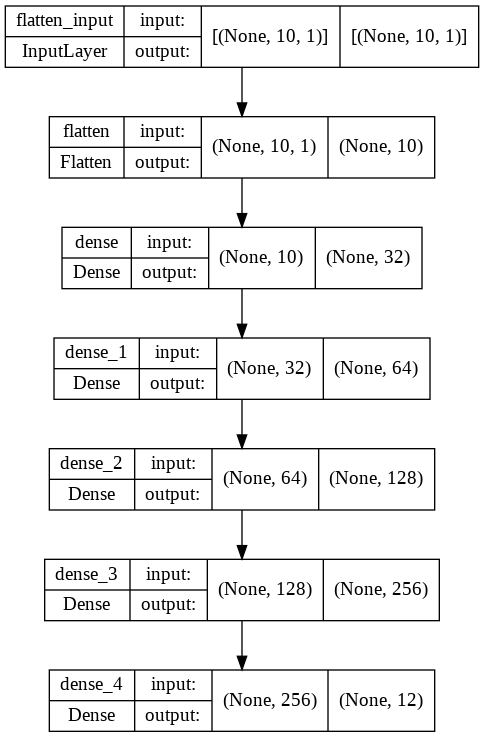
\includegraphics[width=.4\linewidth]{sections/images/section3/network.png}
    \caption{\gls{dnn} Classification network}
    \label{fig:model_dnn}
\end{figure}